%
% Шаблон для НИР
%

\documentclass[a4paper,12pt]{article}
\usepackage[backend=biber,sorting=none,style=gost-numeric]{biblatex} % библиография
\usepackage{mathtext} %русские буквы в формулах
\usepackage[T2A]{fontenc}
\usepackage[utf8]{inputenc}
\usepackage[english,russian]{babel}
\usepackage{amsmath}
\usepackage{fancyvrb}
\usepackage{formular}
\usepackage{setspace} % управление междустрочными интервалами
%поля документа
\usepackage[left=3cm,right=1cm,top=2cm,bottom=2cm]{geometry}

\usepackage{misccorr} % точки в конце номеров разделов, использовать перед пакетом ccaption!
\usepackage{ccaption} % изменения подписей к рисункам и табл.

\usepackage[nooneline]{caption} 
\captionsetup[table]{justification=raggedright} % заголовок таблицы выравнивается влево
\captionsetup[figure]{justification=centering,labelsep=endash} % заголовок рисунка - по центру

% отступ перед первым абзацем
\usepackage{indentfirst}
%вставка изображений
\usepackage{graphicx}
% счетчики
\usepackage{totcount}
% управление содержанием
\usepackage{tocloft}
% управление таблицами и рисунками
\usepackage{float}

%для добавления количества источников в реферат - не работает для bibtex!
\newtotcounter{citnum} %From the package documentation
\def\oldbibitem{} \let\oldbibitem=\bibitem
\def\bibitem{\stepcounter{citnum}\oldbibitem}

% окружение для листингов - с нумерацией строк слева
\DefineVerbatimEnvironment{MyCode}{Verbatim}{frame=lines,numbers=left,numberblanklines=false,framesep=5mm}

% автоматическая нумерация листингов
\newfloat{Program}{phb}{lop}
\floatname{Program}{Листинг}
\floatstyle{ruled}

\setcounter{secnumdepth}{3} % глубина нумерации до подразделов

%если нужны точки в оглавлении для разделов - раскомментируйте следующую команду
%\renewcommand{\cftsecleader}{\cftdotfill{\cftdotsep}}

\addto\captionsrussian{%
\renewcommand{\figurename}{Рисунок}%
\renewcommand{\tablename}{Таблица}%
}

% дефис в подписи к рисункам
\captiondelim{ -- } 

% Настройки для окружений с подчеркиваниями для подписей и пр.
\setFRMfontencoding{T2A}
\setFRMdfontencoding{T2A}
% thanks to A.Starikov
\setFRMfontfamily{cmr}
\setFRMdfontfamily{ptm}
\setFRMdfontsize{10pt}

% задает длину поля для подписи на титульной странице
\newFRMfield{xtitlesign}{32mm}

% поле для факультета или кафедры
\newFRMfield{fcath}{65mm}

%имя файла с библиографией в формате BibTex
\addbibresource{rbiblio.bib}

\begin{document}

% счетчики страниц, рисунков, таблиц
\regtotcounter{page}
\regtotcounter{figure}
\regtotcounter{table}

\renewcommand{\refname}{\centerline{СПИСОК ИСПОЛЬЗОВАННОЙ ЛИТЕРАТУРЫ}} 
\renewcommand{\contentsname}{\centerline{СОДЕРЖАНИЕ}} 
%\renewcommand{\refname}{Список источников}  % По умолчанию "Список литературы" (article)
%\renewcommand{\bibname}{Литература}  % По умолчанию "Литература" (book и report)

% титульная страница
\thispagestyle{empty}
\begin{center} \small
\textbf{МИНИСТЕРСТВО ОБРАЗОВАНИЯ И НАУКИ РОССИЙСКОЙ ФЕДЕРАЦИИ}\\
ФЕДЕРАЛЬНОЕ ГОСУДАРСТВЕННОЕ АВТОНОМНОЕ ОБРАЗОВАТЕЛЬНОЕ УЧРЕЖДЕНИЕ
ВЫСШЕГО  ОБРАЗОВАНИЯ\\
«Национальный исследовательский ядерный университет «МИФИ»\\
\textbf{Обнинский институт атомной энергетики} – \\
филиал федерального государственного автономного образовательного учреждения высшего\\
образования «Национальный исследовательский ядерный университет «МИФИ»\\
(ИАТЭ НИЯУ МИФИ)
\end{center}
%\vfill
\medskip

% Направление подготовки следует уточнять,
% магистры и бакалавры могут иметь разные наименования
\begin{center}
\begin{tabular}{rl}
Отделение & \useFRMfield{fcath}[\large Интеллектуальные кибернетические системы] \\ 
Направление подготовки & \useFRMfield{fcath}[\large Информационные системы и технологии] \\ 
\end{tabular} 
\end{center}

\vfill

\large 

\begin{center}
	Научно-исследовательская работа \\
	
	\medskip
	
	\textbf{\Large 
		Разработка мобильного приложения для преобразования 2D фотографий в 3D вид
	}
	
\end{center}

\vspace{1cm}

\begin{tabular*}{\textwidth}{lcr}
Студент группы ИС-Б14 & \useFRMfield{xtitlesign} & А.В.Кузнецов\\
& & \\
Руководитель & & \\
к.т.н., доцент отделения ИКС & \useFRMfield{xtitlesign} & О.А.Мирзеабасов\\
\end{tabular*}


\vfill
\large

\begin{center}
Обнинск, 2017 г
\end{center}

\onehalfspacing

\pagebreak

% реферат
\thispagestyle{empty}

\section*{\centering РЕФЕРАТ}

% возможно, кол-во источников придется вставлять вручную
\total{page} стр., \total{figure} рис. , 4 ист. 

ANDROID, JAVA, МОБИЛЬНОЕ ПРИЛОЖЕНИЕ, ПОЛЬЗОВАТЕЛЬСКИЙ ИНТЕРФЕЙС, КАРТА ГЛУБИНЫ, АНАЛИЗ, 3D, АНИМАЦИЯ, GIF

Настоящая работа посвящена изучению методов получения трехмерных изображений из двумерных и разработке пользовательского интерфейса мобильного приложения для преобразования 2D фотографий в 3D вид. 

Разработанная программа дает возможность преобразовывать простую фотографию в объемную картинку, в виде GIF.

\pagebreak
\thispagestyle{empty}

\section*{\centering ОПРЕДЕЛЕНИЯ}

Референсы --- изображения или другие ресурсы для разработки графического интерфейса с учетом существующих, успешно работающих решений

\pagebreak

\section*{\centering ОБОЗНАЧЕНИЯ И СОКРАЩЕНИЯ}


UI (user interface) --- пользовательский интерфейс\\
UX (user experience) --- пользовательский опыт\\
ПО –-- программное обеспечение\\



\pagebreak



\tableofcontents
% если нужно добавить "Стр." над номерами страниц - раскомментируйте следующую команду
%\addtocontents{toc}{~\hfill\textbf{Стр.}\par}

\pagebreak

\section*{\centering ВВЕДЕНИЕ}
\addcontentsline{toc}{section}{ВВЕДЕНИЕ}
Основным результатом выполнения проекта будет мобильное приложение, предназначенное для преобразования 2D изображений в 3D вид. Приложение будет распространяться с помощью его размещения в Google Play (для Android-устройств). Соответственно, в качестве основных потребителей создаваемой продукции следует рассматривать владельцев мобильных устройств, которые любят использовать свой телефон или планшет в качестве фотоаппарата. Более того, то подмножество этих пользователей, которые, помимо фотографирования, активно обрабатывают свои фото средствами мобильного устройства и активно делятся этими результатами с друзьями посредством соцсетей.

Поэтому главной целью текущей НИР является изучение разработки мобильного приложения, работы алгоритма преобразования двумерных изображений в трехмерные и разработке современного, функционального и удобного пользовательского интерфейса. 

Задачи, решаемые в ходе работы (в соответствии с заданием на НИР):
\begin{enumerate}
	\item Изучение основ разработки мобильного приложения в среде Android Studio;
	\item Основные компоненты пользовательского интерфейса мобильного приложения в Android;
	\item Проектирование структуры приложения;
	\item Разработка мобильного приложения;
	\item Изучение работы алгоритма определения глубины изображения;
	\item Подготовка отчета и презентации по НИР.
\end{enumerate} % текст введения в файле intro.tex
\pagebreak

%\input{Post_zad}
\pagebreak
% первая часть

\section{Описание предметной области}
В ходе выполнения проекта, главным образом, решается задача преобразования двумерных изображений в трехмерные(GIF) на мобильных устройствах.

В последние годы заметное место в области преобразования и фильтрации изображений занимает задача преобразования двумерных изображений в трехмерные. На сегодняшний день в мире для этого разработаны различные методики, которые позволяют автоматически создавать так называемые «карты глубины» для двумерных изображений, основываясь на свойствах этого изображение и на некоторых предположениях о характере сцены. 

\subsection{Android Studio}
Android Studio - полностью укомплектованная платформа для разработки и тестирования приложений под операционную систему Android. Разработчики этой оболочки (компания Google) внедрили весь необходимый инструментарий для удобного и качественного проектирования новых приложений и доработки существующих. Программа включает в себя такие компоненты как Android SDK, все версии операционки Android, эмулятор для запуска приложений, элементы тестирования и отладки программ.

Создавая новый проект, будет доступна полная структура приложения со всеми файлами, что позволяет более четко и продуманно организовать сам процесс разработки. Очень удобно реализован показ вносимых изменений и дополнений - визуально в реальном времени происходят преобразования в зависимости от заданных действий. Что немаловажно, программа позволяет делать разработку приложений для всех версий ОС Andriod и для различных устройств - можно предварительно оценить внешний вид программы, например, под планшет или смартфон.

Среда Android Studio предназначена как для небольших команд разработчиков мобильных приложений (даже в количестве одного человека), или же крупных международных организаций с GIT или другими подобными системами управления версиями. Опытные разработчики смогут выбрать инструменты, которые больше подходят для масштабных проектов. Решения для Android разрабатываются в Android Studio с использованием Java или C++. В основе рабочего процесса Android Studio заложен концепт непрерывной интеграции, позволяющий сразу же обнаруживать имеющиеся проблемы. Продолжительная проверка кода обеспечивает возможность эффективной обратной связи с разработчиками. Такая опция позволяет быстрее опубликовать версию мобильного приложения в Google Play App Store. В Android Studio есть удобная маркировка кода, которая позволит без труда ориентироваться в больших проектах. Кроме того, отдельные компоненты можно изменять простым перетаскиванием в другое нужное место, что значительно упрощает редактирование.

\subsection{Java}
Преимущества языка Java
\begin{itemize}
	\item Одно из основных преимуществ языка Java — независимость от платформы, на которой выполняются программы: один и тот же код можно запускать под управлением операционных систем Windows, Solaris, Linux, Machintosh и др. 
	Это действительно необходимо, когда программы загружаются через Интернет для последующего выполнения под управлением разных операционных систем.
	\item Другое преимущество заключается в том, что синтаксис языка Java похож на синтаксис языка C++, и программистам, знающим языки С и C++, его изучение не составляет труда.
	\item Кроме того, Java — полностью объектно-ориентированный язык, даже в большей степени, чем C++. Все сущности в языке Java являются объектами, за исключением немногих основных типов (primitive types), например чисел.
	\item Исключена возможность явного выделения и освобождения памяти.	Память в языке Java освобождается автоматически с помощью механизма сборки мусора. Программист гарантирован от ошибок, связанных с неправильным использованием памяти.
	\item Безопасный: методы проверки подлинности основаны на шифровании с открытым ключом.
	\item Динамический: программирование на Java считается более динамичным, чем на C или C++, так как он предназначен для адаптации к меняющимся условиям. Программы могут выполнять обширное количество во время обработки информации, которая может быть использована для проверки и разрешения доступа к объектам на время выполнения.
\end{itemize}

\subsection{Выбор архитектуры мобильного приложения}
В ходе выполнения работы были рассмотрены различные варианты для создания мобильных приложений, предназначенных для преобразования 2D изображений в 3D вид. При этом рассмотрении учитывалось, что результирующие мобильные приложения должны создаваться под операционные системы Android, а также то, что один из основных результатов работы приложения с точки зрения конечного пользователя – это возможность публикации созданного 3D-изображения в виде анимированного gif-файла в одном или нескольких аккаунтов в социальных сетях пользователя. Соответственно, можно исходить из предположения о том, что для функционирования приложения в любом случае необходим доступ к сети интернет. Максимальная унификация различных составных частей приложения между собой хотя бы на уровне исходных кодов вне зависимости от целевой платформы (Android или iOS) является дополнительным преимуществом при рассмотрении различных вариантов создания мобильных приложений.

Один из наиболее простых с технической точки зрения вариантов реализации решения, позволяющего преобразовывать 2D файлы в 3D вид, является решение, основанное на создании веб-сервиса, который предоставляет минимально необходимый пользовательский интерфейс для загрузки желаемого файла на сервер, преобразования файла на сервере и, как результат, возможность скачать получившийся файл на устройство пользователя и поделиться этим файлом в социальных сетях. При простоте архитектуры у этого решения есть один существенных недостаток – как правило, такие решения менее удобны и функциональны, чем нативные (native) мобильные приложения, разработанные специально под целевую платформу, на которой они будут функционировать.

Рассмотрим два варианта создания нативных мобильных приложений:

\begin{enumerate}
	\item Использовать наиболее популярные средства разработки и языки программирования для каждой из необходимых мобильных платформ. Создать нативное мобильное приложение, реализующее весь необходимый пользовательский интерфейс, набор сервисных функций. Портировать алгоритм преобразования графического файла из 2D в 3D для локального исполнения на мобильном устройстве. Все необходимые преобразования выполнять локально, на мобильном устройстве. Полученный результат преобразования (анимированный gif) загружать в интернет (социальные сети) по мере его готовности на мобильном устройстве.
	
	\item Использовать наиболее популярные средства разработки и языки программирования для каждой из необходимых мобильных платформ для создания нативных мобильных приложений только для реализации пользовательского интерфейса и набора сервисных функций. Алгоритм преобразования графического файла из 2D в 3D реализуется в виде серверного модуля, соответственно для преобразования выбранного файла и предварительного просмотра полученных результатов необходимо загрузить этот выбранный файл на сервер. Загрузить полученный результат с сервера и поделиться этим результатом в социальных сетях.
\end{enumerate}

Для варианта №1 для операционной системы Android необходимо:

С использованием Android Studio на языке программирования Java реализовать необходимый пользовательский интерфейс, а также весь необходимый набор сервисных функций. Необходимо адаптировать реализацию алгоритма преобразования графического файла из 2D в 3D для использования под управлением операционной системы Android (реализация на С++). Далее, с использованием механизма The Android Native Development Kit (NDK) необходимо обеспечить вызов кода, написанного на языке С++ из «классического» Android-приложения. 

Для реализации варианта №2 необходимо:

С использованием Android Studio на языке программирования Java необходимо создать нативное мобильное приложение для реализации пользовательского интерфейса и набора сервисных функций. Эта задача, в целом, является типовой и принципиальных сложностей не вызывает. Алгоритм преобразования графического файла из 2D в 3D следует реализовать в виде серверного модуля, например, для использования под управлением операционной системы Ubuntu. Это обусловлено тем, что Unix-подобные операционные системы имеют существенно более широкое распространение в Web-серверном окружении, чем Windows-сервера.

На основе проведенного исследования моно сделать следующий вывод. С точки зрения скорости, легкости и качества реализации наиболее перспективными являются вариант №2. 

Очевидным недостатком подобного решения является существенная его зависимость от скорости и надежности мобильного интернета, а также от доступности конечному пользователю оплаченного траффика. Для обхода этих ограничений предполагается исследовать возможность создания для пользователей ОС Android «самодостаточного» мобильного приложения (вариант №1), которое все необходимые действия, связанные с преобразованием файлов производит непосредственно на мобильном устройстве.

\section{Изучение основ разработки мобильного приложения в среде Android Studio}

Android основан на Linux. Между приложением и ядром лежит слой API и слой библиотек на нативном коде. Приложение выполняется на виртуальной машине Java (Dalvik Virtual Machine).
В Android можно запускать много приложений. Но одно из них есть главным и занимает экран. От текущего приложения можно перейти к предыдущему или запустить новое. Это похоже на браузер с историей просмотров.

Каждый экран пользовательского интерфейса представлен классом Activity в коде. Различные Activity содержатся в процессах. Activity может даже жить дольше процесса. Activity может быть приостановлена и запущена вновь с сохранением всей нужной информации.(рисунок~\ref{fig:activity})

\begin{figure}[H]
	\centering
	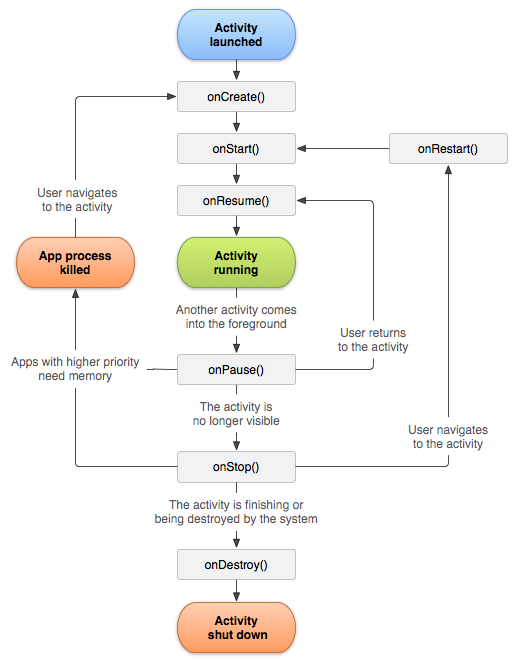
\includegraphics[width=0.6\linewidth]{pics/activity}
	\caption{activity}
	\label{fig:activity}
\end{figure}

Android использует специальный механизм описания действий основанный на Intent. Когда нужно выполнить действие (сделать звонок, послать письмо, показать окно), вызывается Intent.

Также Android содержит сервисы подобные демонам в Linux для выполнения нужных действий в фоновом режиме (например, проигрывание музыки).
Для обмена данными между приложениями используются Content providers (провайдеры содержимого).

Содержимое Activity формируется из различных компонентов, называемых View. Самые распространенные View - это кнопка, поле ввода, чекбокс и т.д. (рисунок~\ref{fig:view})

\begin{figure}[H]
	\centering
	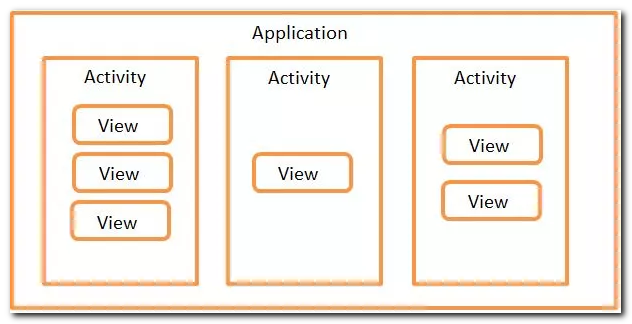
\includegraphics[width=0.6\linewidth]{pics/view}
	\caption{view}
	\label{fig:view}
\end{figure}

Необходимо заметить, что View обычно размещаются в ViewGroup. Самый распространенный пример ViewGroup – это Layout. Layout бывает различных типов и отвечает за то, как будут расположены его дочерние View на экране.

LinearLayout – отображает View-элементы в виде одной строки (если он Horizontal) или одного столбца (если он Vertical).

TableLayout – отображает элементы в виде таблицы, по строкам и столбцам.

RelativeLayout – для каждого элемента настраивается его положение относительно других элементов.

AbsoluteLayout – для каждого элемента указывается явная позиция на экране в системе координат (x,y)

\section{Основные компоненты пользовательского интерфейса мобильного приложения в Android}

В Android используется UI-фреймворк, сравнимый с другими полнофункциональными UI-фреймворками, применяемыми на локальных компьютерах. Он является более современным и асинхронным по природе. По существу, UI-фреймворк Android относится уже к четвертому поколению, если считать первым поколением традиционный прикладной интерфейс программирования Microsoft Windows, основанный на С, а MFC (Microsoft Foundation Classes, библиотека базовых классов Microsoft на основе C++) - вторым. В таком случае UI-фреймворк Swing, основанный на Java, будет третьим поколением, так как предлагаемые в нем возможности дизайна значительно превосходят по гибкости MFC. Android UI, JavaFX, Microsoft Silverlight и язык пользовательских интерфейсов Mozilla XML (XUL) относятся к новому типу UI-фреймворков четвертого поколения, в котором UI является декларативным и поддерживает независимую темизацию.

При программировании в пользовательском интерфейсе Android применяется объявление интерфейса в файлах XML. Затем эти определения представления (view definitions) XML загружаются в приложение с пользовательским интерфейсом как окна. Даже меню приложения загружаются из файлов XML. Экраны (окна) Android часто называются активностями (activities), которые включают в себя несколько видов, нужных пользователю, чтобы выполнить логический элемент процесса. Виды (views) являются основными элементами, из которых в Android состоит пользовательский интерфейс. Виды можно объединять в группы (view groups). Для внутренней организации видов используются давно известные в программировании концепции холст (canvas), рисование (painting) и взаимодействие пользователя с системой (user interaction).

Такие составные представления, в которые входят виды и группы видов, работают на базе специального логического заменяемого компонента пользовательского интерфейса Android.

Одной из ключевых концепций фреймворка Android является управление жизненным циклом (lifecycle) окон явлений (activity windows). В системе применяются протоколы, поэтому Android может управлять ситуацией по мере того, как пользователи скрывают, восстанавливают, останавливают и закрывают окна явлений.


\section{Проектирование структуры приложения}

Одна из важнейших задач в ходе создания мобильного приложения, преобразовывающего 2D снимки в объемные (3D) - разработка удобного и интуитивно-понятного пользовательского интерфейса. UI/UX (user Interface, user experience) составляющая, она же пользовательский интерфейс и пользовательский опыт, является более чем просто значимым элементом современного мобильного приложения. Удобство расположения элементов управления и приятное визуальное оформление напрямую влияют на настроение пользователя при использовании продукты. Именно некачественный UI/UX-дизайн отпугивает людей от использования многих приложений в пользу их более достойных альтернатив.

На главный экран камеры (рисунок~\ref{fig:Artboard}) выведены следующие функции:

\begin{itemize}
	\item Спуск затвора;
	\item Выбор фото из галереи;
	\item Смена камеры;
	\item Управление вспышкой;
	\item Переход к настройкам и справке.
\end{itemize}

\begin{figure}[H]
	\centering
	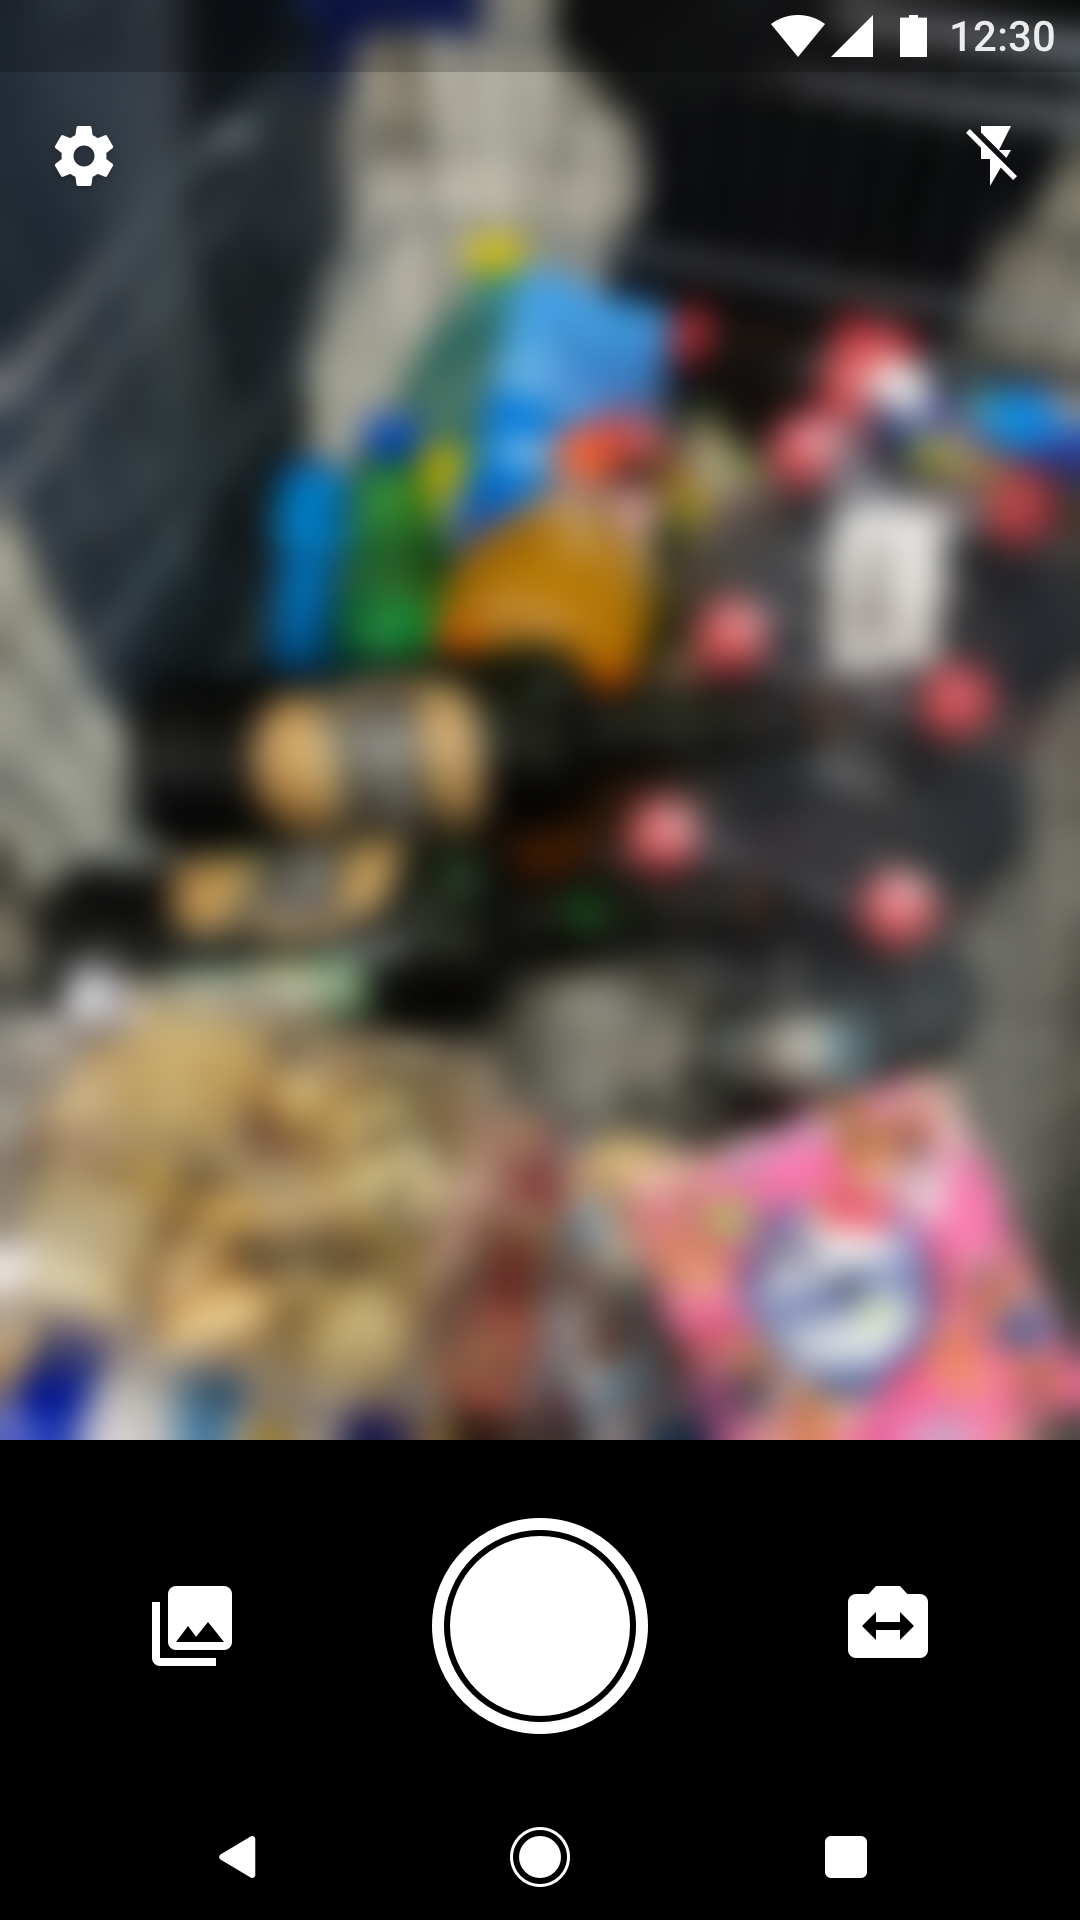
\includegraphics[width=0.6\linewidth]{pics/Artboard}
	\caption{Окно с камерой}
	\label{fig:Artboard}
\end{figure}

На экране с обработанной фотографией по нажатии кнопки «Далее» появляется bottom sheet (рисунок~\ref{fig:Artboard2}), включающий в себя быстрые функции шеринга и сохранения полученного фото в галерею.

\begin{figure}[H]
	\centering
	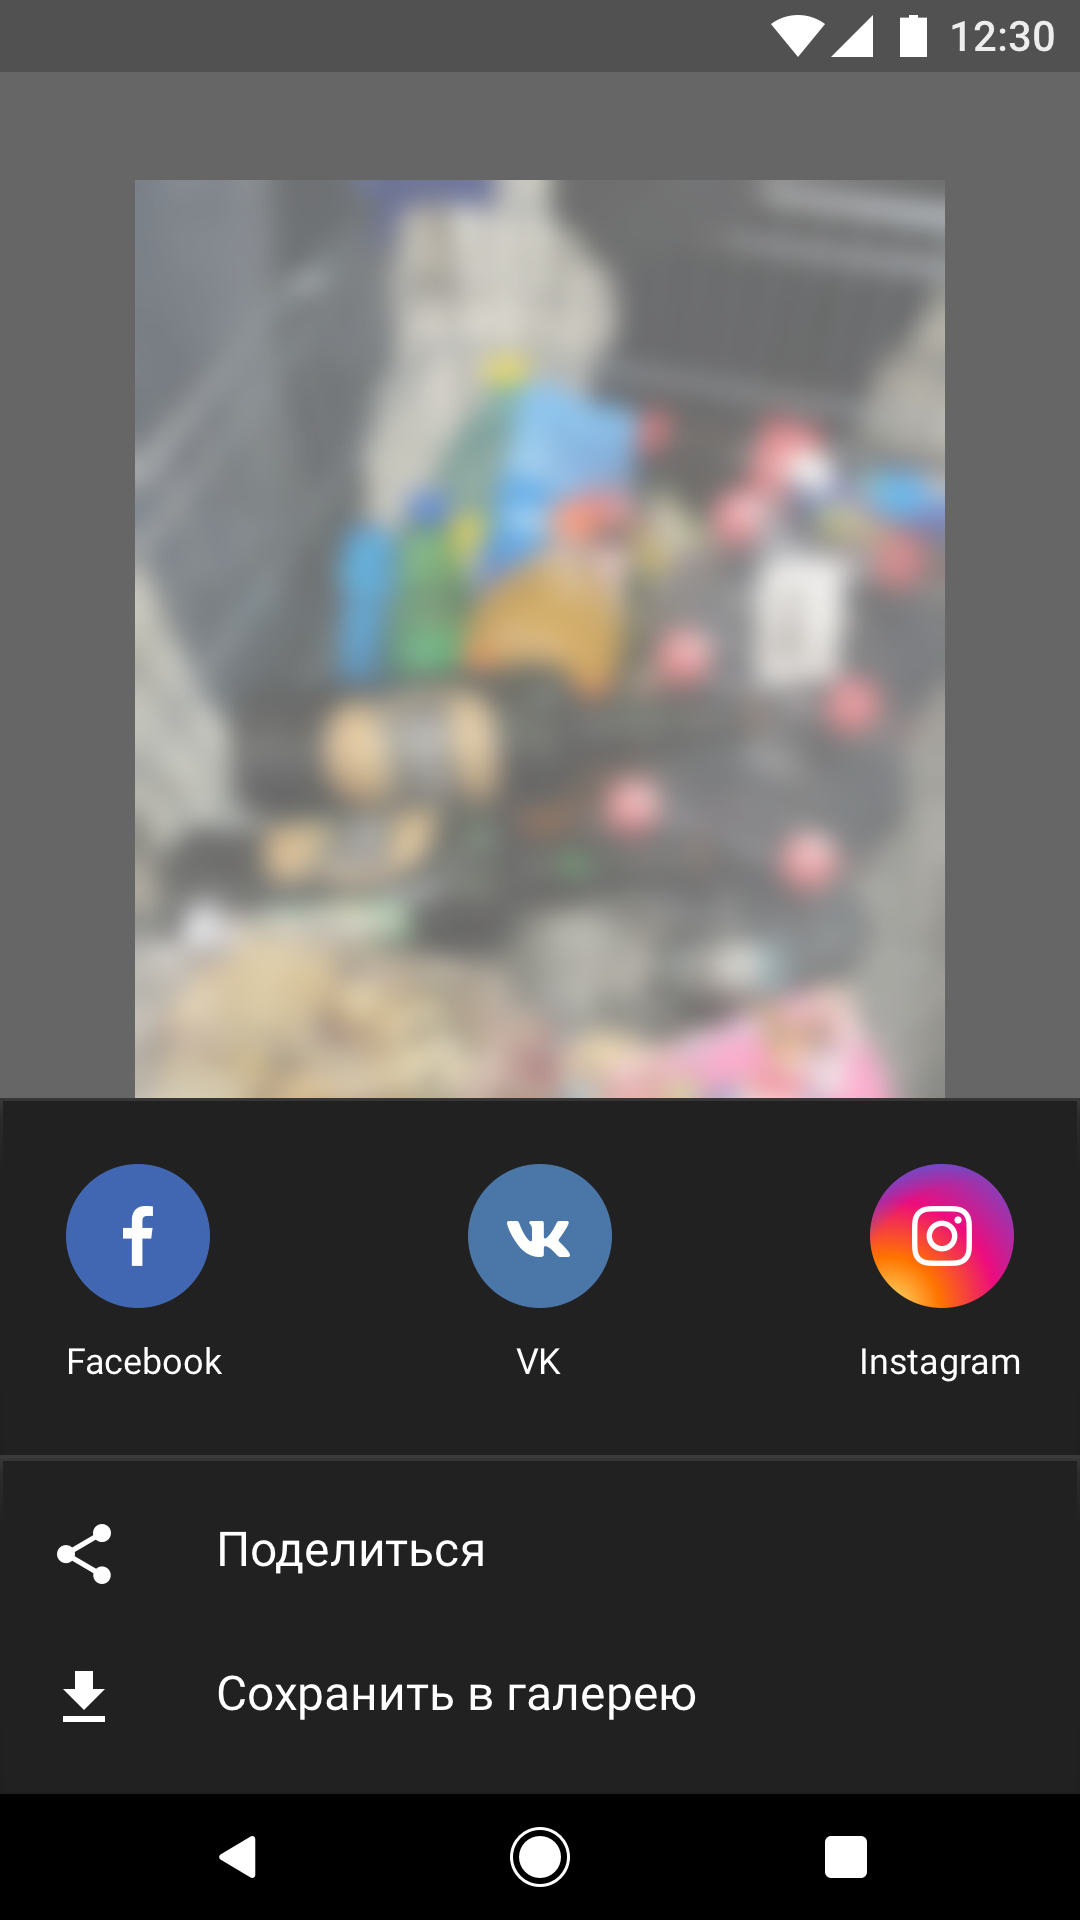
\includegraphics[width=0.6\linewidth]{pics/Artboard2}
	\caption{Окно с просмотром фото}
	\label{fig:Artboard2}
\end{figure}

При создании пользовательского интерфейса приложения были проанализированы современные, с аналогичным функционалом мобильные приложения в целом. Был сделан акцент на необходимости создания современного, функционального и не перегруженного пользовательского интерфейса. В результате проведенного анализа был создан пользовательский интерфейс мобильного приложения для преобразования 2D фотографий в 3D вид.

\section{Разработка мобильного приложения}



  % первая глава - в файле part1.tex
\pagebreak
% вторая часть

\section{Восстановление глубины из одного расфокусированного изображения}

В этой главе мы рассмотрим сложную задачу восстановления глубины из одного расфокусированного изображения. Мы представляем простой, но эффективный подход для оценки объема пространственно изменяющегося размытия в краевых положениях. Входное расфокусированное изображение повторно размыто с использованием гауссова ядра, а значение размытости размытия может быть получено из коэффициента градиента между входными и повторно размытыми изображениями. Распространяя количество размытия в крайних положениях на все изображение, можно восстановить всю карту глубины сцены. % вторая глава - в файле part2.tex
\pagebreak

% если есть еще разделы - сохраните их в соответствующих файлах и раскомментируйте строки ниже, при необходимости добавьте еще
%\input{part3}  % третья глава - в файле part3.tex
%\pagebreak

%\input{part4} % четвертая глава - в файле part4.tex
%\pagebreak

%\input{part5}  % пятая глава - в файле part5.tex
%\pagebreak

\section*{\centering ЗАКЛЮЧЕНИЕ}
\addcontentsline{toc}{section}{ЗАКЛЮЧЕНИЕ}

В ходе проделанной работы изучил основы разработки мобильного приложения в среде Android Studio. Также была изучена работа алгоритма определения глубины изображения.

При создании пользовательского интерфейса приложения был сделан акцент на необходимости создания современного, функционального и не перегруженного пользовательского интерфейса. В результате  было создано мобильное приложение, с помощью которого можно сделать снимок и сохранить его в галерею.

% оформление библиографии - вариант с БД
\pagebreak

\addcontentsline{toc}{section}{СПИСОК ИСПОЛЬЗОВАННОЙ ЛИТЕРАТУРЫ}
% ВАЖНО: для корректного отображения в списке литературы ссылок на англ.языке в bibtex-описание источника следует добавить поле 
% langid = {english}
\printbibliography

\pagebreak

\section*{ \centering Приложение А} 
\addcontentsline{toc}{section}{Приложение А}

\begin{center}
Листинг 1 -- Часть кода реализации класса \verb|MainActivity|
\end{center}


\begin{MyCode}

public class MainActivity extends AppCompatActivity {
	
	ImageView ivPreview;
	String mCurrentPhotoPath;
	@Override
	protected void onCreate(Bundle savedInstanceState) {
		super.onCreate(savedInstanceState);
		setContentView(R.layout.activity_main);
		ivPreview = findViewById(R.id.image);
		Button btn = findViewById(R.id.button);
		btn.setOnClickListener(new View.OnClickListener() {
			@Override
			public void onClick(View v) {
				dispatchTakePictureIntent();
			}
		});
	}
	
	private void dispatchTakePictureIntent() {
		Intent pictureIntent = new Intent(
		MediaStore.ACTION_IMAGE_CAPTURE);
		Intent pictureIntent2 = new Intent(
		MediaStore.ACTION_IMAGE_CAPTURE);
		if(pictureIntent.resolveActivity(getPackageManager()) != null){
			//Create a file to store the image
			File photoFile = null;
			try {
				photoFile = createImageFile();
			} catch (IOException ex) {
				// Error occurred while creating the File
				
			}
			if (photoFile != null) {
				Uri photoURI = FileProvider.getUriForFile(this, getPackageName(), photoFile);
				Intent mediaScanIntent = new Intent(Intent.ACTION_MEDIA_SCANNER_SCAN_FILE);
				File f = new File(mCurrentPhotoPath);
				mediaScanIntent.setData(photoURI);
				this.sendBroadcast(mediaScanIntent);
				pictureIntent.putExtra(MediaStore.EXTRA_OUTPUT,
				photoURI);
				startActivityForResult(pictureIntent2,
				1);
			}
		}
	}
	
	private File createImageFile() throws IOException {
		// Create an image file name
		String timeStamp = new SimpleDateFormat("yyyyMMdd_HHmmss").format(new Date());
		String imageFileName = "JPEG_" + timeStamp + "_";
		File storageDir = getExternalFilesDir(Environment.DIRECTORY_PICTURES);
		File image = File.createTempFile(
		imageFileName,  /* prefix */
		".jpg",         /* suffix */
		storageDir      /* directory */
		);
		
		// Save a file: path for use with ACTION_VIEW intents
		mCurrentPhotoPath = image.getAbsolutePath();
		return image;
	}
	
	
	@Override
	protected void onActivityResult(int requestCode, int resultCode, Intent data) {
		if (requestCode == 1 && resultCode == RESULT_OK) {
			Bitmap imageBitmap = (Bitmap) data.getExtras().get("data");
			ivPreview.setImageBitmap(imageBitmap);
		}
	}
}
\end{MyCode}

\end{document}          

